% Admissible: a fail-closed admissibility kernel for non-replayable generators.
% Self-contained arXiv preprint. Built with pdflatex (see Makefile).
\documentclass[11pt,a4paper]{article}

\usepackage[T1]{fontenc}
\usepackage[utf8]{inputenc}
\usepackage[margin=1in]{geometry}
\usepackage{amsmath,amssymb,amsthm}
\usepackage{booktabs}
\usepackage{longtable}
\usepackage{graphicx}
\usepackage{float}
\usepackage{lmodern}
% Protrusion only: font expansion needs expandable font sets that a minimal
% TeX Live install may not carry, and arXiv compiles the source itself.
\usepackage[protrusion=true,expansion=false]{microtype}
\usepackage{enumitem}
\usepackage[hidelinks]{hyperref}
\usepackage{cleveref}

\theoremstyle{plain}
\newtheorem{theorem}{Theorem}
\newtheorem{lemma}{Lemma}
\theoremstyle{definition}
\newtheorem{definition}{Definition}
\theoremstyle{remark}
\newtheorem*{remark}{Remark}

\newcommand{\adm}{\ensuremath{\mathrm{admissible}}}
\newcommand{\norm}{\ensuremath{\mathrm{norm}}}
\newcommand{\SR}{\ensuremath{S_R}}
\newcommand{\code}[1]{\texttt{#1}}

\title{Admissible: A Fail-Closed Admissibility Kernel for\\Work Products of Non-Replayable Generators}

\author{%
  Roque Brice\~no\\
  \small Independent researcher, PRIV\'E, S.\ de R.L., Honduras\\
  \small \texttt{roque@priveperfumeshn.com}\\
  % Replace with the author's ORCID iD before submission; arXiv links it from
  % the abstract page and it is the only stable identifier an independent
  % researcher has.
  \small ORCID: 0000-0000-0000-0000
}

\date{\today}

\begin{document}
\maketitle

\begin{abstract}
A software integrity mechanism that identifies \emph{which} component ran normally tells you \emph{what} it did. That inference fails for a large language model: the same worker, prompt and context yield a different artifact on each run, so an accepted output cannot be certified by naming its author. We present Admissible, a reference monitor for work products of such generators, built as three fail-closed transition systems --- identity, scrutiny and standing --- composed by non-interference, whose combined guarantee is the soundness of a single query over an append-only record, $\adm(\mathit{id})$, together with the loudness of its complement. Identity proves that a stage completed only on the model bound from a class-scoped allow set, with no fallback edge. Scrutiny proves that an artifact sealed only when pre-registered, deterministic, replayable refuters --- pinned before generation and measured against named defect models --- were given a fair chance to falsify its claims and failed, with the measured power carried on the seal as a kernel-counted primary and never raised afterwards. Standing proves that a defect found in sealed work, demonstrated as a counterfactual re-run of the very instrument the seal trusted, mechanically impeaches that seal, charges every vouching refuter, and cannot be silently forgotten by a successor policy.

The guarantees are about the \emph{record}, never about truth: what is proved is that the paperwork cannot lie about who ran, what was survived at what measured strength, and what has been found against it since. We report two results beyond the construction. First, an asymmetry theorem for revocation: standing falls by a demonstration alone and rises only past an attributed, journaled act, which is strictly stronger than the revocation infrastructures the design descends from. Second, a verification methodology --- every guard an individually deletable named method with a red-first deletion proof, every proof step bound to a live source line by a move-detecting test --- which we applied to our own released kernel and which located five soundness defects in it, including one that let a single party un-impeach every artifact a checker had impeached. We give the repairs, the resulting theorem statements, and the residue that remains open.
\end{abstract}

\section{Introduction}
\label{sec:intro}

Delegating work to a stochastic generator breaks the oldest assumption in software integrity: that knowing which component ran tells you what it did. A deterministic function's identity determines its output; an agent's does not. Three questions follow, in order, and each is the subject of one layer of the system described here.

\begin{enumerate}[leftmargin=*,itemsep=2pt]
  \item \textbf{Who did the work?} Control planes name one model while data planes call another; a dead bind can silently continue on a fallback; a reviewer can be the author. Without identity nothing downstream is attributable.
  \item \textbf{What was the work subjected to before acceptance?} A green check from an empty test suite and one from a suite that kills 95\% of seeded defects print identically. Survival without measured severity launders weak scrutiny into strong.
  \item \textbf{What happens when accepted work turns out to be wrong?} In most pipelines, nothing mechanical. The miss is fixed, the instruments that vouched keep vouching, and the next battery is free to forget the defect class.
\end{enumerate}

\subsection{The predicate}

The system's guarantees compose into one query, which the implementation exposes and which we define here:
\begin{equation}
  \adm(\mathit{id}) \;\triangleq\; \mathit{id} \in \SR \;\wedge\; \mathrm{mediated}(\mathit{id}) \;\wedge\; \neg\,\mathrm{tainted}(\mathit{id}) \;\wedge\; \neg\,\mathrm{impeached}(\mathit{id}),
  \label{eq:pred}
\end{equation}
where $\SR$ is the sealed store, written only by the Seal transition, which itself requires the identity layer's Accept; \emph{mediated} means the standing authority counter-signed this seal in the same step it was issued; \emph{tainted} means a refuter the seal relied on was later caught nondeterministic; and \emph{impeached} means a valid escape stands against a sealed claim. Each conjunct is the top of one theorem family.

The name is an argument as well as a label. Evidence law admits testimony not because it is true but because it satisfies procedure: established provenance and custody, a known error rate, controlling standards, and exposure to cross-examination, with impeachment available afterwards. The \emph{Daubert} factors for expert evidence~\cite{daubert} --- testability, known or potential error rate, maintenance of standards --- map onto this kernel directly: refuters are the testability requirement, carried power is the known error rate (a claim about the \emph{instrument}, never about the generator's real-world error rate), pinned versioned policy is the controlling standard, and the escape ledger is impeachment. The analogy is honest precisely where the theorems are: admissibility certifies procedure, never truth, and the seal says so on its face.

\subsection{Contributions}

\begin{enumerate}[leftmargin=*,itemsep=3pt]
  \item A three-layer fail-closed transition system in which identity, scrutiny and standing are each enforced by a kernel with inductive safety invariants, composed by two non-interference lemmas so that each layer's proofs survive composition unchanged (\Cref{sec:layers,sec:composed}).
  \item \textbf{Measured doubt as a carried record} (\Cref{sec:scrutiny}). Power enters a seal only as a kernel-counted kill rate against a content-addressed defect model, or as a computed bound from declared, seal-visible parameters; never as a scalar a caller wrote down. Composition across refuters is by measured union or labelled maximum, never a product, and the two sorts are never collapsed into one another --- so a declared figure cannot clear a floor that a measurement failed.
  \item \textbf{Escapes as counterfactual trials, and an asymmetry theorem for revocation} (\Cref{sec:standing,sec:composed}). A post-acceptance defect report is a re-run of the \emph{pinned} refuter at a finder-chosen input, adding no trust assumption the seal did not already carry. From it: non-discretionary impeachment, per-cell charge totality, a coverage ratchet on policy succession, and query-shaped demotion. We prove that standing falls by demonstration alone and rises only past an attributed, journaled act (\Cref{thm:asym}).
  \item \textbf{A verification methodology, and what it found in our own kernel} (\Cref{sec:method,sec:findings}). Every guard is an individually deletable named method with a red-first deletion proof; every proof step cites a live source line, bound by a move-detecting test. Applying the discipline to the released kernel located five soundness defects, one of which falsified a published theorem. We report them and the repairs rather than only the successes.
  \item An explicit boundary stated as the theorems' complement (\Cref{sec:limits}): what is not proved, the two empirical hypotheses the numbers rest on, and every trust assumption (\Cref{app:assumptions}).
\end{enumerate}

\paragraph{What is not new.} The access-control skeleton is Clark and Wilson's integrity model~\cite{clarkwilson} with fail-safe defaults~\cite{saltzer} and Anderson's reference-monitor triad~\cite{anderson}; this stack is their model completed for non-replayable workers rather than a new algebra, and we say so at each layer. Measured scrutiny is mutation analysis~\cite{demillo,jiaharman,just} and property testing~\cite{ggr}; concordance is the zero-entropy corner of semantic entropy~\cite{kuhn,farquhar}; the standing layer's shape is certificate revocation~\cite{rfc5280} and Assurance 2.0 defeater discipline~\cite{bloomfield}. \Cref{sec:related} gives the deltas, and \Cref{sec:limits} the non-claims.

\section{Setting and threat model}
\label{sec:setting}

\paragraph{Parties.} An \emph{operator} owns policy and adjudication: trusted for governance, made visible, not defeated (B13). \emph{Specialists} (generators) are untrusted and non-replayable. \emph{Refuters} are deterministic programs under a pinned hermetic runtime (B2). A \emph{harness} executes and reports, honest per B1/A10 --- the classical adapter boundary. \emph{Finders} of escapes are untrusted; their filings are checkable.

\paragraph{On ``stochastic''.} The property the theorems consume is not that a generator samples from a distribution. No theorem here uses a measure over generator outputs, and every quantity the kernel carries is a primary precisely because it refuses to put one there. The load-bearing dichotomy is \emph{replayability}: a component is replayable if its outputs are a function of journaled roots, so every claim about it can be re-derived by anyone holding the record, and non-replayable otherwise, so every claim about it is either a demonstration that was run or a report that is believed. Generators are non-replayable by nature; refuters are \emph{required} to be replayable and are refused when caught otherwise. That is the asymmetry the whole design exploits.

\paragraph{Machines.} Three state machines with disjoint write sets, composed left to right by read-only observation and guarded interposition:
\[
  \mathcal{F}\ (\text{identity}) \;\longleftarrow\; \mathcal{A}\ (\text{scrutiny}) \;\longleftarrow\; \mathcal{L}\ (\text{standing}).
\]
$\mathcal{A}$ reads $\mathcal{F}$'s state and writes none of it (R11); $\mathcal{L}$ reads both and writes neither directly, driving $\mathcal{A}$ only through its own guarded transitions (C7). Every transition appends to an append-only journal, and every machine rebuilds deterministically from its journal, re-checking on rebuild what it checked live. \Cref{fig:composition} states the predicate and the layers it decomposes into.

\begin{figure}[H]
  \centering
  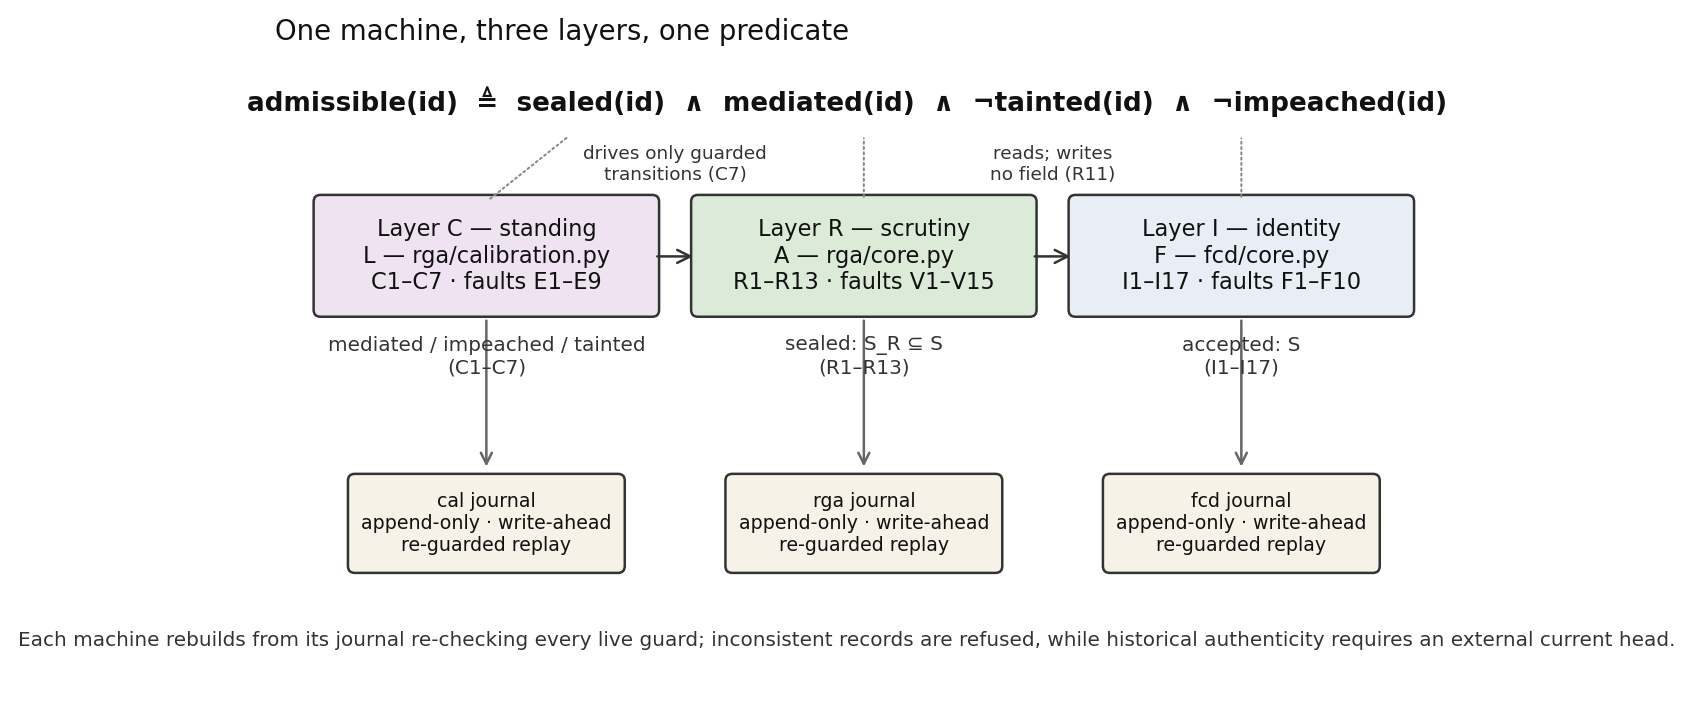
\includegraphics[width=0.82\textwidth]{fig1-composition.png}
  \caption{The composed machine. Each conjunct of $\adm$ is the top of one theorem family, and each layer answers exactly one of \Cref{sec:intro}'s three questions.}
  \label{fig:composition}
\end{figure}

\paragraph{Adversary.} In scope: any sequence of public transitions by untrusted parties --- mis-binding, fallback hopping, claim-shaping, refuter-shaping, tailoring outputs to known tests, witness multiplication, corpus flooding with true filings, inconsistent journal tampering detected at replay, and selection across retries. Out of scope, and stated as assumptions in \Cref{app:assumptions}: physical execution fidelity (A10/B1), runtime hermeticity (B2), hash second-preimage resistance (A11/B7), author-identity strings (B11), operator governance (B13), authenticated-publication key and registry integrity (B14), and post-seal byte availability (B12). Coherent history replacement or deletion is detected only relative to a previously trusted authenticated publication; \Cref{sec:composed} states that residue precisely, and \Cref{sec:findings} widens it by one event class as the price of a repair.

\section{The three layers}
\label{sec:layers}

\subsection{Identity}
\label{sec:identity}

A work item carries a class $c$ and a frozen body. Policy gives each class an allow set $\pi(c)$ and a deny set $\delta(c)$, disjoint, and binds each specialist $a$ to one API model identity $\phi(a)$; display strings are compared after normalisation. On a check stage the effective allow set excludes the item's authors. The machine's rows are Open, Admit, Bind, Observe, Pass/PassRefuse, Close, Retry and Accept, with the load-bearing split that \textbf{Bind writes only the declared identity and Observe alone writes the executed one}, so the Pass guard $\norm(m_{\mathrm{exec}}) = \norm(m_{\mathrm{decl}})$ compares two independently sourced witnesses and can genuinely fail (\Cref{fig:writers}). Retry, where a class has one, is the same item on a specialist not yet tried; it does not search a leftover fallback list.

\begin{figure}[H]
  \centering
  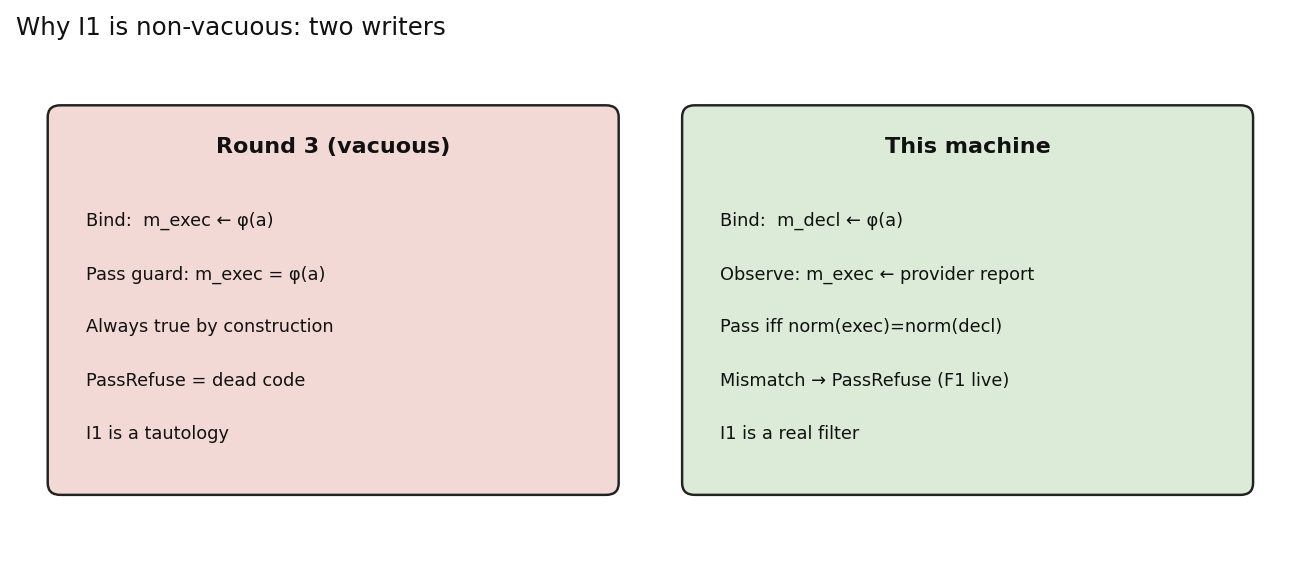
\includegraphics[width=0.66\textwidth]{fig2-writers.png}
  \caption{Why I1 is not vacuous. A table in which one transition writes both identities makes the Pass guard a tautology; separating the writers is what gives the guard two independently sourced witnesses to compare, and it is the single most important structural decision in this layer.}
  \label{fig:writers}
\end{figure}

\begin{theorem}[Identity, selected clauses]
\label{thm:identity}
On the identity machine, under A0--A13:
\begin{enumerate}[label=\textup{I\arabic*},leftmargin=2.2em,itemsep=1pt]
  \item $\mathit{pc} = \mathrm{Passed} \Rightarrow \norm(m_{\mathrm{exec}}) = \norm(m_{\mathrm{decl}}) = \norm(\phi(a))$.
  \item[I3] No Passed state has $\norm(m_{\mathrm{exec}})$ outside $\{\norm(\phi(x)) : x \in \pi^{*}(c)\setminus\delta(c)\}$: this table has no leftover-hop edge.
  \item[I5] $\mathit{status} = \mathrm{accepted} \Rightarrow$ every required stage of $c$ has Passed.
  \item[I6] On a check-stage admit, $a \notin \mathit{authors}$: dual control.
  \item[I8] $\mathit{id} \in S \Rightarrow \mathit{status} = \mathrm{accepted}$, and $S$ has exactly one writer.
\end{enumerate}
Invariants I10--I17 additionally pin the context envelope: package hashes, receipts, steering acknowledgement and cache identity all bind to the current attempt and nonce, and project memory promotes only through serialised compare-and-swap by accepted work. Full statements and proofs are in \Cref{app:identity}.
\end{theorem}

This layer is Clark--Wilson's enforcement rules applied to model binds --- constrained data items, transformation procedures, validated writes, separation of duty --- and claims no new access-control algebra. Item liveness does not hold, and there is no quality theorem.

\subsection{Scrutiny}
\label{sec:scrutiny}

Identity verifies the die, not the roll. The scrutiny layer moves the gate to the claim. A class pins, at Open and \emph{before any generation}: formal claims identified by spec hash (the generator never authors what it is measured against), the refuter versions that attack each claim, a sample count $k$, a concordance threshold $\theta$, and a power floor $p_{\min}$.

\begin{definition}[Samples, trials, power, concordance]
A \emph{line} is one identity-layer work item whose first $k$ stages are write stages under one bind key. A \emph{sample} is such a stage after identity Pass; the kernel hashes the bytes it is handed and draws a nonce afterwards, so identity is inherited per sample by citation of I1--I3. A \emph{trial} is one refuter against one claim on one sample, seeded by $H(\nu_i \Vert h_i \Vert r \Vert \mathit{claim})$, so no seed exists before the artifact it attacks; verdicts are \emph{refuted}, \emph{survived} or \emph{inconclusive}, and only survival counts. \emph{Power} enters only as a record, in one of two sorts: \emph{ledger}, where the kernel counts kills over a ledger of per-defect verdicts against a content-addressed defect model $D$ whose id-set and author are fixed by first record, exact on $D$; or \emph{bounded}, $1-(1-\varepsilon)^N$ computed from a declared $(\varepsilon,N)$ the seal carries. \emph{Concordance} for a claim is the agreement of witness vectors with the \emph{designated} sample --- stage $0$, fixed before anything ran --- a precondition that closes the gate, never an election.
\end{definition}

\begin{theorem}[Scrutiny]
\label{thm:scrutiny}
Under B0--B11, R1--R13 are inductive on the combined machine. In particular:
\begin{enumerate}[label=\textup{R\arabic*},leftmargin=2.4em,itemsep=1pt]
  \item $\mathit{id} \in \SR \Rightarrow$ every $(\mathit{claim}, \mathit{refuter}, \mathit{sample})$ cell has a trial with verdict \emph{survived}, and no trial on the line was refuted or inconclusive; the latter two close the line, published.
  \item Power is carried, never inferred: every figure on a seal equals a write-once record the kernel computed; nothing raises it afterwards; composition across refuters is measured union over a shared $D$ or a labelled maximum, never a product. The two sorts occupy separate fields, and the floor is compared against the \emph{weaker} sort present (\Cref{sec:floor}).
  \item Separation of duty, extended: the refuter was fixed before generation, authored by neither the generator nor the defect model's author; the generator's package provably excluded refuter material; and samples were interleaved with their stages, so slots cannot be assigned after seeing the batch.
  \item[R4] Concordance against the designated sample at $\theta$, with $(\mathit{agreeing},k)$ on the seal, so $k=1$ is visibly trivial.
  \item[R5] A replay divergence refuses a refuter monotonically, everywhere.
  \item[R6] Every refuter used was replayed at least once on this line with an identical outcome.
  \item[R8] $\SR \subseteq S$: everything sealed was first accepted by the identity layer.
  \item[R11] $\mathcal{A}$ writes no field of $\mathcal{F}$ --- the first composition lemma.
\end{enumerate}
Statements R7, R9, R10, R12 and R13 and all proofs are in \Cref{app:scrutiny}.
\end{theorem}

The seal carries the artifact hash; per claim, each refuter's mode, power, $D$ or $(\varepsilon,N)$, kills and $|D|$; the composite with its label; the two sorts' own coordinates with the floor basis and the contributor that realised it; $(\mathit{agreeing},k)$; the sampling configuration; the identity-layer identity; the identity-journal position it read; and an explicit list of what was \emph{not} attacked, with its disposition. \Cref{fig:seal} is the whole record.

\begin{figure}[H]
  \centering
  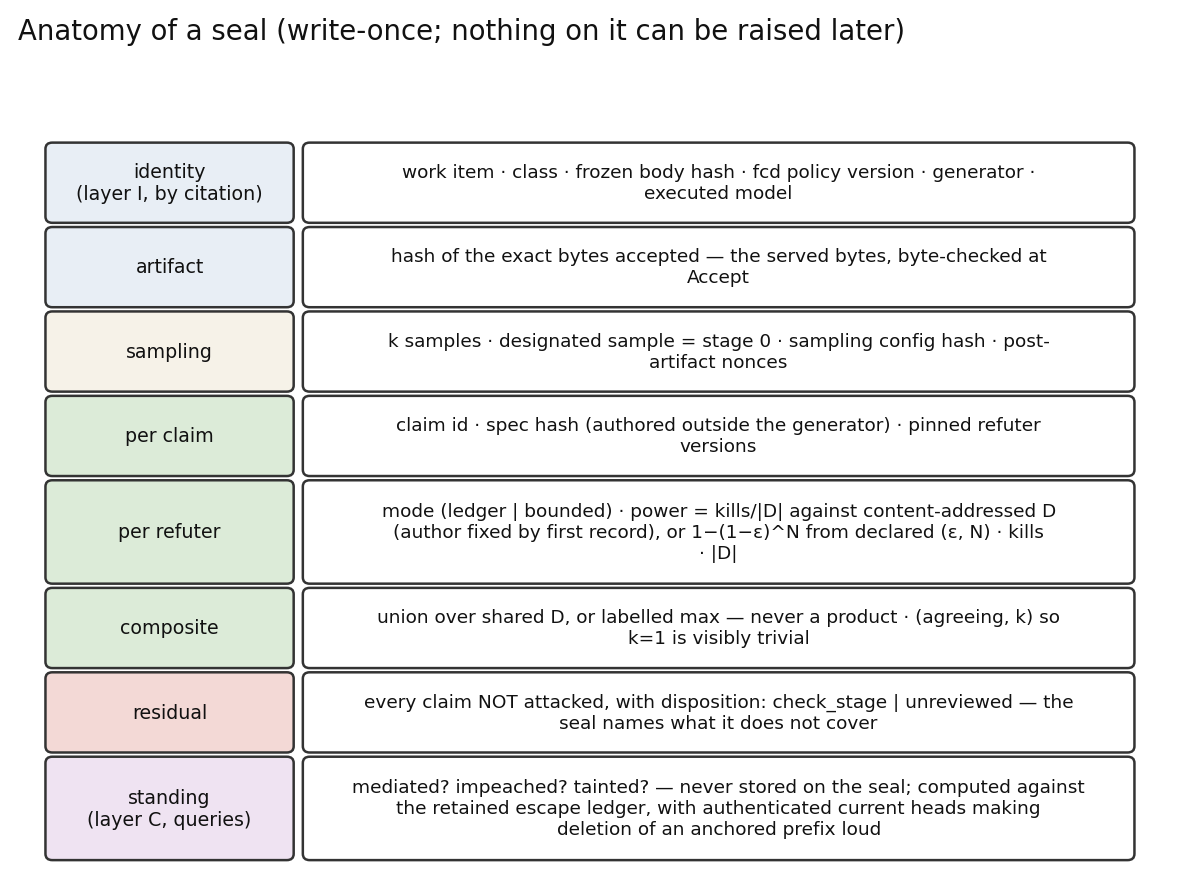
\includegraphics[width=0.80\textwidth]{fig3-seal.png}
  \caption{Anatomy of a seal. Every field is write-once, and nothing on it can be raised afterwards. The residual line is the class's declared list of what was not attacked, which is on the record precisely so that a reader is not left to infer coverage from silence.}
  \label{fig:seal}
\end{figure}

\subsubsection{Why the floor reads the weaker sort}
\label{sec:floor}

A ledger figure is counted by the kernel over a named finite defect set. A bounded figure is computed from a declared failure mass. The two quantify over different alternatives, so a maximum across them is not a lower bound on anything joint. Taking it anyway had a consequence we did not anticipate and which \Cref{sec:findings} reports as a defect: because \code{bound} accepts $(\varepsilon,N) = (1,1)$, whose figure is $1.0$, a declaration could clear any floor on a claim whose kernel-counted power was $0/|D|$ --- a declaration outranking a measurement.

The repair is at the cause rather than the instance. Banning $\varepsilon = 1$ would not do: $(0.9999,10)$ reaches the same figure. Instead the sorts are never collapsed. The seal carries each coordinate separately, and the gate compares
\[
  \mathrm{floor\_basis}_j \;=\; \min \{\,\text{coordinates of the sorts present on claim } j\,\},
\]
so where both sorts attack a claim each must clear the floor on its own base, and $\mathrm{power\_min} = \min_j \mathrm{floor\_basis}_j$ is what a dependency gate reads. A claim attacked only by declarations still clears its floor by declaration --- a kernel cannot measure what nobody measured --- and the recorded witness says so, which is the label a reader needs in order to discount it.

\subsection{Standing}
\label{sec:standing}

Scrutiny leaves one loop open, and its own limits name it: a kill rate on $D$ is power against real defects only under an empirical coupling hypothesis (B6), and nothing forces a found miss to have consequences. The standing layer closes the loop that can be closed.

\begin{definition}[Escape, tier, establishment, contest]
An \emph{escape} against a sealed claim is, in its automatic form (\emph{tier A}), a counterfactual trial: the claim's pinned refuter re-run at a finder-chosen nonce on the sealed bytes. The finder supplies only the nonce and the bytes; the kernel hashes the bytes against the seal, derives the seed itself, and requires verdict \emph{refuted}. Any other checker is \emph{tier B} and has no effect of any kind until a named, journaled adjudication accepts it --- the per-escape claim-fidelity judgement made visible rather than pretended away. An escape is \emph{established} when one replay of it returns an identical verdict and witness. A replay of an established run that \emph{diverges} marks that run \emph{contested}, and a contest is settled by a \emph{resolution}: a named, reasoned decision to uphold or void, journaled once.
\end{definition}

\begin{theorem}[Standing]
\label{thm:standing}
On the standing machine:
\begin{enumerate}[label=\textup{C\arabic*},leftmargin=2.4em,itemsep=1pt]
  \item \textbf{Established, never asserted.} A tier-A escape has effect only past kernel-checked preconditions --- seal membership, byte-hash equality, pinned checker, kernel-derived seed, refuted verdict, identical replay --- none of which is a declaration; a tier-B escape only past an attributed adjudication. The same discipline governs the falsifier: what removes an established escape's effect is a divergence on \emph{that} run plus an attributed resolution, never a report about another run.
  \item \textbf{Charge totality and unit.} Every refuter that vouched is charged --- read from the journal, never declared --- exactly once per $(\mathit{line}, \mathit{claim}, \mathit{refuter\ version})$ cell, so witness and checker multiplicity cannot inflate the count.
  \item \textbf{Impeachment is entailed; un-revocation is attributed.} See \Cref{thm:asym}.
  \item \textbf{The ratchet.} No successor policy installs unless every ledger claim's defect model covers the class's valid corpus minus journaled, attributed exclusions; a class owing coverage cannot be dropped; the install event carries the coverage primaries and the dropped-id diff. Forgetting is loud.
  \item \textbf{Track record carried, mediation provable at both gates.} Every seal issued through the authority is stamped, in the same step, with its instruments' charge record and the corpus's finder-provenance split --- primaries, never a rate, with the stated reading that zero charges is absence of filed evidence --- and every open through the authority journals its own check. $\mathrm{mediated}$ requires both records, so a line that took either transition directly on the lower machine is visibly layer-IR and \Cref{eq:pred} refuses it.
  \item[C6] \textbf{Demotion.} Charges past a declared budget block new pins unconditionally and gate sealing where the class declared it: a pure function of the valid charge set, never an event cascade and never a rewrite of an existing seal.
  \item[C7] $\mathcal{L}$ writes no lower-layer field directly --- the second composition lemma.
\end{enumerate}
Proofs are in \Cref{app:standing}.
\end{theorem}

\section{The composed guarantees}
\label{sec:composed}

The unified results are compositions, proved by citation of the layer theorems plus the two non-interference lemmas.

\begin{theorem}[Soundness of the record]
\label{thm:sound}
If $\adm(\mathit{id})$ holds at journal position $t$, then the journals up to $t$ contain, re-derivably: (i) for each of the $k$ samples, a bind and an observation whose normalised identities agree with $\phi$ of a specialist admitted from $\pi^{*}(c)\setminus\delta(c)$ [I1--I3, via R7]; (ii) for every pinned claim and refuter, a surviving trial on every sample and at least one replayed trial per refuter on this line, seeded after the artifact it attacked, under power records the kernel computed, with concordance $\ge \theta$ against the designated sample and floor basis $\ge p_{\min}$ [R1--R10, R12--R13]; and (iii) no valid escape standing against any sealed claim, no reliance on a refuter caught nondeterministic, and a same-step stamp of every instrument's charge record as of sealing [C1--C3, C5].
\end{theorem}

\begin{proof}[Proof sketch]
Each conjunct of \Cref{eq:pred} is the conclusion of the cited family. R11 and C7 guarantee the families hold on the combined trace, because each upper machine's writes are disjoint from the lower machines' state, so the projection of a combined trace onto a layer is a trace of that layer. Clause (iii) is required by the predicate itself rather than merely emitted beside it: a seal the standing authority never mediated carries no stamp, and $\adm$ refuses it as layer IR rather than IRC.
\end{proof}

\begin{theorem}[Loudness of deviation]
\label{thm:loud}
Every transition sequence that would falsify a conjunct of \Cref{thm:sound} either writes nothing --- a guard refusal --- or appends a named fault to the journal before any effect. Replay is moreover \emph{transition-local}: each machine's rebuild re-checks, before every write, the guards that live execution ran, so derived and output fields altered inconsistently, forged or duplicated transitions, and reordering against preconditions are all refused; and every journal a live machine accepted replays unchanged.
\end{theorem}

\begin{proof}[Proof sketch]
By the fault tables (\Cref{app:faults}) and their executable checks: every scrutiny and standing fault names its enforcing method, and for each method singly the suite demonstrates that the forbidden state is unreachable with it and reached without it. Identity faults are driven to refusal by transition tests over the same table. The replay clause is by inspection of the three rebuild functions, each of which re-drives transitions and compares its regenerated events to the supplied record field by field rather than trusting the file.
\end{proof}

\paragraph{Recomputation is a control total, not an anchor.} It is tempting to read a later event that recomputes a figure over the ledger --- a stamp's track records, a policy install's coverage --- as anchoring the events it counts, and an earlier version of this work did. It does not. Such a figure catches a deleter who removes an earlier event and \emph{fails to update it}; every input to the figure lies inside the journal the deleter holds, so one who prunes, rebuilds their own prefix, reads off exactly the values the verifier will recompute, and writes them into the surviving events replays clean. We report this because it changes the price of a deletion from another line's standing to an afternoon's arithmetic, and because the general form is short enough to state: \emph{any check that is a computable function of the journal is computable by whoever holds the journal.} Only a value the holder cannot recompute --- a signature under a key they do not have, or a digest already published elsewhere --- escapes it.

\paragraph{Unauthenticated-history residue.} \Cref{thm:loud} does not say which internally valid history is the anchored one. A coherent rewrite of root transition inputs, a journal shortened at the tail, and --- by the paragraph above --- \emph{any} coherently removed group once the surviving recomputations are refitted, are each indistinguishable from another honest history to replay alone. Deletion is the direction that can \emph{raise} standing, since dropping an escape un-impeaches its line and dropping a refusal un-taints every seal that relied on it. Replay alone cannot close this. A conditional authenticated-publication theorem does: immutable authority-owned journals are sealed into namespace-scoped ordered heads, successor receipts prove extension of the anchored cumulative chain, the heads are accepted atomically, and the exact heads plus the kernel-derived predicates are bound into one signed receipt, whose verification rejects stale, coherently shortened and longer-forked records. It applies only when callers issue and verify that receipt, and still trusts signer and key custody, registry monotonicity, and the single-writer authority model (B14).

\subsection{An asymmetry theorem for revocation}
\label{sec:asymmetry}

Revocation infrastructures --- certificate revocation lists, online status protocols, transparency logs --- share a standing query of the shape $\mathit{valid} = \mathit{issued} \wedge \neg\mathit{revoked}$, in which deleting a revocation raises standing and a list number is the freshness witness~\cite{rfc5280,kocher,laurie}. What they lack, and what a kernel can supply, is non-discretion: a revocation that carries its own replayable proof cannot be declined. The dual question is less often asked. If revocation is entailed by a demonstration, what entails \emph{un}-revocation?

The honest answer is that it cannot be entailed at all. A replay divergence is a report about a component the system only \emph{assumes} deterministic (B1, B2); when two reports about one run conflict, the kernel has no ground on which to prefer either. Our first design let the later report win silently, and \Cref{sec:findings} records the consequence. What a kernel can do is refuse the silence.

\begin{theorem}[Asymmetry of standing]
\label{thm:asym}
Let $\mathrm{valid}$ be the standing layer's query over a filed run. Then
\begin{enumerate}[leftmargin=*,itemsep=1pt]
  \item \emph{(Downward, non-discretionary.)} $\mathrm{impeached}(\mathit{id})$ is entailed by the existence of a valid refuted run against a claim of $\SR[\mathit{id}]$. The seal is never rewritten, no field of it is assignable, and no transition of any layer can decline the entailment.
  \item \emph{(Upward, attributed.)} The only path from $\mathrm{valid}$ to $\neg\mathrm{valid}$ for an \emph{established} run is: a replay of \emph{that} run whose reported verdict and witness diverge from the filed pair, which marks it contested and leaves it impeaching; followed by a resolution event deciding \emph{void}, carrying a named actor and a reason. No single report, about any other run or from any other layer, raises a line's standing.
\end{enumerate}
\end{theorem}

\begin{proof}[Proof sketch]
Downward is immediate: the query is a read over the filed runs and the validity predicate, and the latter consults nothing an issuer controls. Upward is by enumerating the writers of every field the validity predicate reads. Establishment falls to no transition, since nothing assigns it false. The resolution field is written by exactly one transition, past a guard requiring a contest, no prior resolution, a decision in $\{\mathrm{uphold},\mathrm{void}\}$, and a nonempty actor and reason. The contested field is written by exactly one transition, on a divergent replay of that same run, and only when the run had already established. The tier-B adjudication field gates tier B alone and can never turn a valid run invalid. Hence the sole valid-to-invalid path is a divergence on the run itself followed by a \emph{void} resolution; both are journaled and the second is attributed. The full proof, with the writer inspection, is in \Cref{app:standing}.
\end{proof}

\begin{remark}
A contested but unresolved escape keeps impeaching. That is the fail-closed direction for the artifact and the aggressive direction for the instrument, and both are deliberate: a suspect checker's demonstrated kill is not cleared by a report about the checker itself. The cost is stated in \Cref{sec:findings}.
\end{remark}

\section{Verification discipline}
\label{sec:method}

This is engineering discipline rather than a verification technique, and it is worth a section because it is what located the defects in \Cref{sec:findings}. We say what it is not first: the guards are Python, the proofs are prose, and the citation binder is a text search. Machine-checked refinement of a kernel against its specification~\cite{sel4} is a strictly stronger form of the same goal, and a reader entitled to ask ``why not verify it?'' should have the comparison from us rather than have to make it.

\paragraph{Delete the guard.} Every guard of the scrutiny and standing kernels is a named method. For each, the suite runs a scenario twice: with the guard intact, in which the forbidden state must be unreachable, and with the guard replaced by a no-op, in which it must be reached. A guard that no deletion turns red fails the suite as dead code, and the discipline is applied to itself --- clauses proved unreachable by construction are removed and derived instead, with the removal recorded. There are $47$ such per-guard proofs and $2$ joint cuts for theorems that two guards enforce together. The identity kernel predates this discipline: its guards are driven to refusal by transition tests over the same fault table, without per-guard deletion.

The argument is \emph{first-order}, and the distinction matters because the section could otherwise be read as an adequacy claim. Deleting each guard singly proves each individually necessary. It does not prove the registered scenarios minimal, nor that every violation class whose minimal cut lies inside the guard basis is registered: two size-two cuts of the scrutiny kernel --- a sealed line with more than $k$ samples, and a sealed line whose pinned refuter was refused before Open and so escapes the taint query --- are reachable only by deleting a pair, and are absent from the joint registry. Higher-order adequacy in the sense of~\cite{higherorder} is not claimed.

\paragraph{Bind the citations.} Every scrutiny and standing proof step cites a \code{file:line:symbol} triple, and two tests open the file and fail if the line no longer contains the symbol. This is a move-detector, not a semantic check: the sentence claims enforcement, and the test keeps the sentence pointed at live code. It fired during the work reported here, which is the point --- and it is worth recording that the naive repair is wrong. When lines shift, re-pointing each citation at the nearest line containing its symbol lands on docstrings, decorators and call sites rather than enforcing lines. Carrying the citations along an exact old-to-new line map, computed by diffing against the previous revision, moved $195$ of them correctly and left exactly the ones on genuinely edited lines for a human.

\paragraph{Attack the premise before the kernel.} Each layer's design brief was attacked by independent adversarial reviewers \emph{before} any code was written, with every finding handed to a skeptic instructed to refute it. Two pre-registered designs were killed at that stage --- a Wilson-interval power bound, and sibling-item sampling --- which is the cheap time to kill them. The finished kernels were then re-attacked, and all confirmed findings applied with red-first tests.

\section{What the methodology found in our own kernel}
\label{sec:findings}

We applied the discipline to the released kernel by computing the \emph{polarity} of its event alphabet: for the standing query, which event types can only raise it, which can only lower it, and which are neutral. An event that raises a standing predicate is a candidate soundness defect, since the design intends exactly one such event class. The computation located five defects. We report them because a methodology's value is what it catches, and because two of them falsified sentences we had published.

\paragraph{F1: a single party could un-impeach everything a checker had impeached.} A divergent replay by a checker discredited it, and the validity predicate voided \emph{every} run of that checker, established or not. One party holding the sealed bytes could therefore file a junk tier-A escape, self-replay it divergently, and lift every impeachment that checker had established --- with nothing tainted and an empty refusal set. This contradicted the published non-discretion claim, and our own transition table had always said only \emph{unestablished} escapes were void. A second channel had the same shape through the scrutiny layer's refusal registry. The repair is \Cref{thm:asym}: a discredit or refusal voids only what a checker never demonstrated, and since an unestablished run already fails the establishment clause, neither set appears in the validity predicate at all. What reaches an established escape is a contest on that run and an attributed resolution.

\paragraph{F2: a declaration could clear a floor a measurement failed.} Described in \Cref{sec:floor}.

\paragraph{F3 and F4: two halves of one replay seam.} The standing layer's rebuild re-checked one filing guard against the \emph{final} registry, so an honest journal whose checker was refused \emph{later} was refused on rebuild; and it omitted the refusal check the live guard makes, so a filing by an already-refused checker was refused live and accepted on rebuild. The repair records the cut: a filing carries the scrutiny-journal position it was written at, and rebuild evaluates the checker's standing there. Because a recorded position is a root on replay, it is bounded rather than trusted --- at or after the seal it files against, at or before the end of the journal, and never earlier than an earlier filing's --- which converts a free choice into a coherent rewrite of the surrounding record. That is a narrowing, not a closure, and it is the same residue every recorded position in this stack carries.

\paragraph{F5: mediation was provable at one gate but claimed for two.} The predicate's \emph{mediated} conjunct read the seal's stamp alone. Because the open transition emitted no event, two things followed, and the second is the defect. C6's open-time demotion gate was never re-verified on rebuild; and a line opened \emph{around} the authority, and therefore never subjected to that gate, could be sealed \emph{through} it and answer \emph{mediated} on the strength of the stamp. A consumer had no way to see that half the mediation never happened. This is not the documented consumer-redirection boundary --- that boundary says a deployment which bypasses the authority gets the lower layer's guarantees, and \emph{mediated} exists precisely to make the bypass visible --- it is the query over-promising. The open transition now journals its check after the delegated transition succeeds, so a refused open leaves no trace, and \emph{mediated} requires both records. This strengthens an existing conjunct rather than adding one, so \Cref{thm:sound} reads unchanged.

This is also where we learned not to trust a control total. Deleting an open event does make a later stamp fail to recompute, and we briefly recorded that as the event being \emph{anchored}. It is not: by the paragraph on control totals in \Cref{sec:composed}, a deleter who refits the surviving stamps replays clean. What the repair rests on is the guard, not the arithmetic --- an absent open event makes the line layer-IR, which is the direction a missing mediation record must fail in.

\paragraph{A cost, stated.} Closing F1 removed an \emph{accidental} anchor. While a refusal voided the refused checker's established escapes, later stamps and policy installs recomputed against it and therefore anchored it: deleting a refusal group changed what a subsequent event re-derived, and replay refused the deletion. Now that validity never reads the refusal registry, no standing reader depends on a refusal, and a refusal group's only remaining effect is the taint it places on seals that pinned the refuter after sealing --- which deleting it removes. Refusal groups are therefore freely deletable by whoever holds the record, and the deletion is invisible to replay alone. The unauthenticated-history residue of \Cref{sec:composed} is one event class wider than before, and closing it takes the authenticated publication path rather than replay. We prefer the wider residue to the fail-open revocation it replaces, and we record the trade rather than only the repair.

\section{Evaluation protocol and results}
\label{sec:eval}

Rates are computed only on a named cut with a class-derived window, from a write-ahead journal, with policy evaluated as-of each event; otherwise zeros are estimates biased clean rather than results. Under that rule the repository carries three studies of decreasing internal validity and increasing external relevance. \textbf{None of them is a claim about any model, and none is part of the gate.}

\paragraph{A kernel bench.} All three layers are driven over reference implementations of four library-specified functions, with the standard library as the strong refuter's differential oracle and a seeded syntax-tree mutator building the defect models. Its numbers are kernel queries on the named cut, reproduced byte-identically by a test. Two of its three generator conditions are close to definitional, and the record says so: the honest sample \emph{is} the reference implementation that serves as the oracle, so its sealing rate is true by construction, and the sloppy mutant is drawn from the very defect model that power is measured against, so its refutation is a within-model result. What the bench does establish is that the machinery is internally consistent under adversarial conditions, plus one thing that is not definitional: every latent-defect seal was impeached afterwards, $7$ of $7$, while three unstable seals were not and stand as misses. That is the standing layer working, and its residue, on the same figure (\Cref{fig:bench}).

\begin{figure}[H]
  \centering
  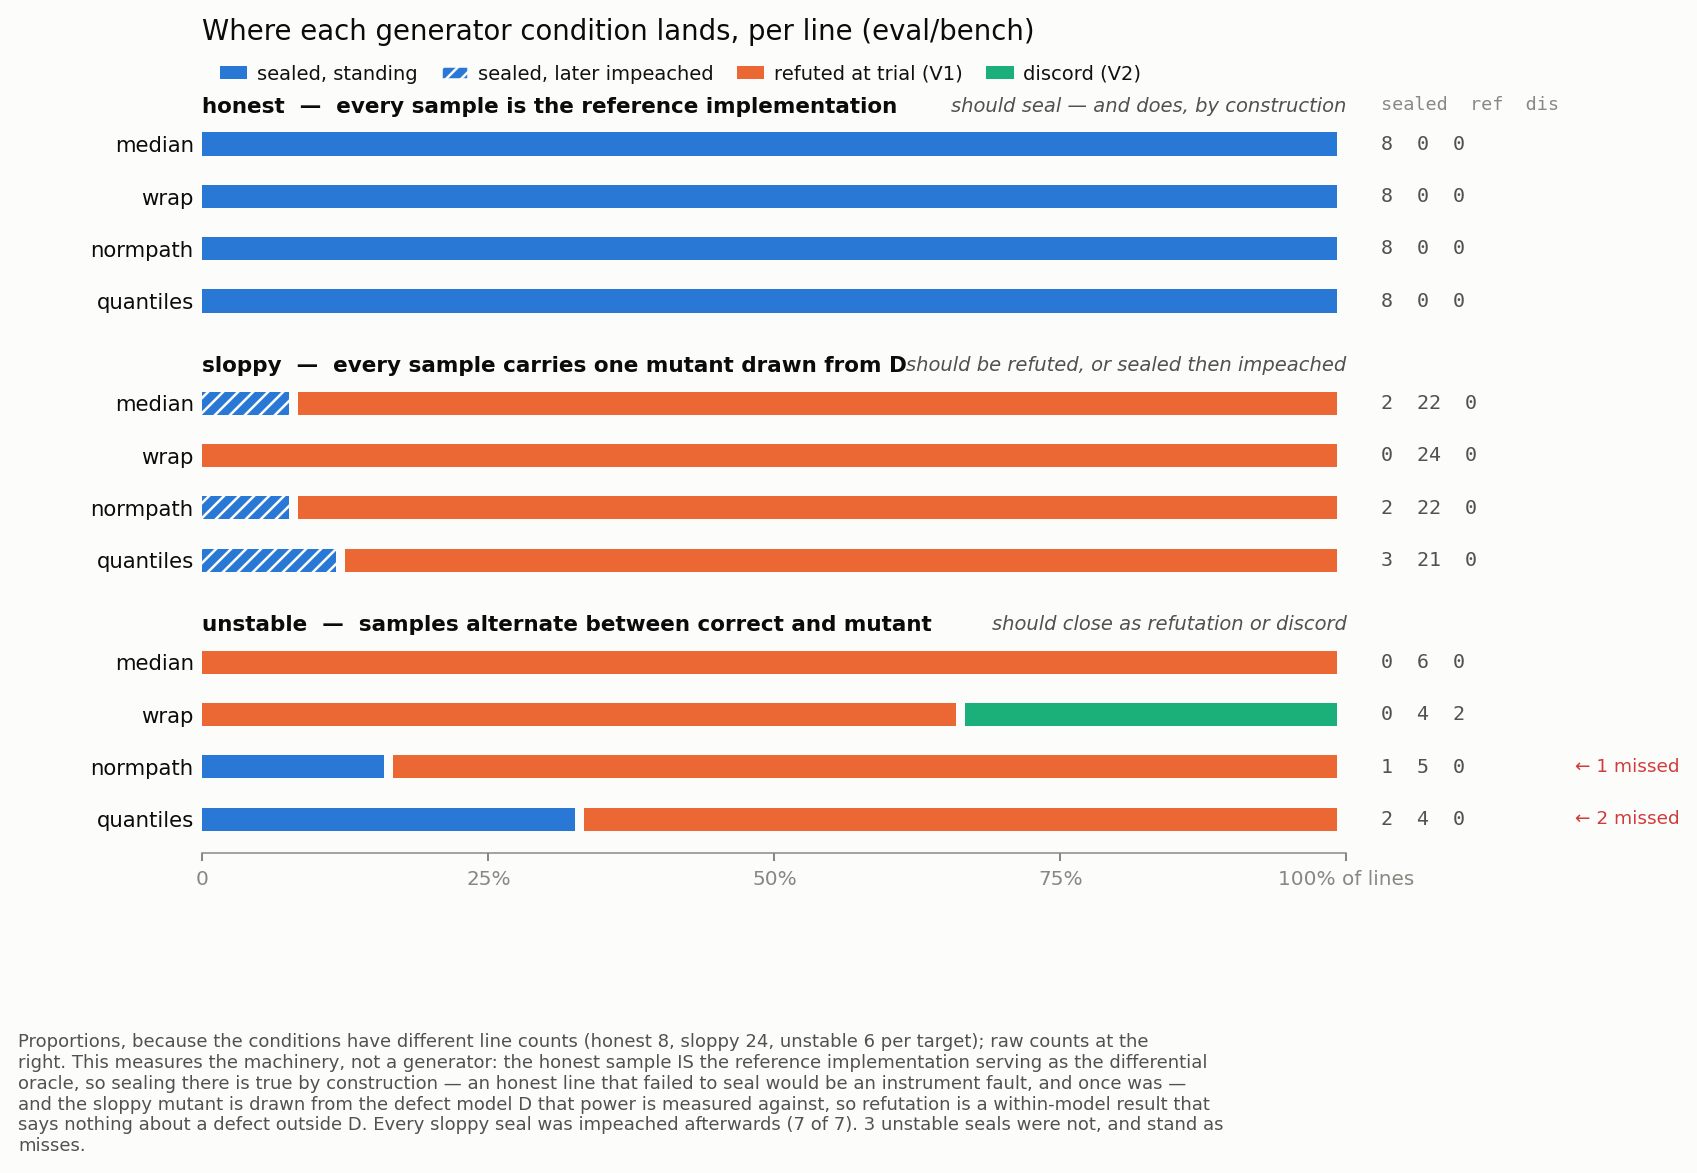
\includegraphics[width=0.86\textwidth]{fig4-bench.png}
  \caption{Where each generator condition lands. The figure labels which cells are true by construction rather than leaving the reader to discover it: the honest sample \emph{is} the differential oracle, and the sloppy mutant is drawn from the very defect model power is measured against. Only the impeachment column is a result.}
  \label{fig:bench}
\end{figure}

\paragraph{A real generator.} A language model replaced the simulated generator for $48$ samples across those four targets, recorded into content-addressed corpora and replayed through the same seam so determinism survives. \emph{Not one sample was defective}: across $12$ textually distinct implementations of one target, all $48$ matched their oracle on $3{,}000$ generated inputs. The gate refused none of them --- $16$ of $16$ lines sealed, zero false refusals --- which is the first measurement of the false-positive half against code a generator actually wrote. It must be read with the corpus's own limitation: nothing recorded establishes that the $k$ samples within a line were independent draws, so concordance is untested there and the discord path is not exercised. The detection half could not be measured, and the reason is structural rather than a matter of adding targets: a target whose oracle is a well-known library function is one whose answer a modern generator recalls rather than derives, so the differential refuter ends up comparing the oracle to itself.

\paragraph{Real historical defects.} The study that bears on the coupling hypothesis directly draws $63$ module-level functions from a curated real-bug corpus, of which $42$ could be run as a differential between their buggy and fixed commits under one interpreter, with inputs found by search rather than sampling and with no knowledge of the bug. It yields \emph{eight defects separated and then hand-verified against the patch that closed them}, each with a re-runnable witness. It does \emph{not} yield a detection rate, and the figure is drawn to refuse one. Five successive runs each carried an instrument fault invisible in its own summary statistic --- a stubbed parent package that cost two thirds of the corpus, a filter too narrow, an argument mutated between the two sides, a filter too broad, and an artifact rule that later measurement showed never fires. Of the last run's $42$ testable candidates, three are excluded by a guard bug rather than by the corpus, two of ten separations are not the documented defect, and of six negatives adjudicated by hand three were overturned by an input written after reading the patch: ``not separated'' mostly means ``not reached''. The honest deliverable is the verified cases and a characterised instrument, and \Cref{fig:realdefects} is drawn to show where the corpus went rather than to invite a ratio out of it.

\begin{figure}[H]
  \centering
  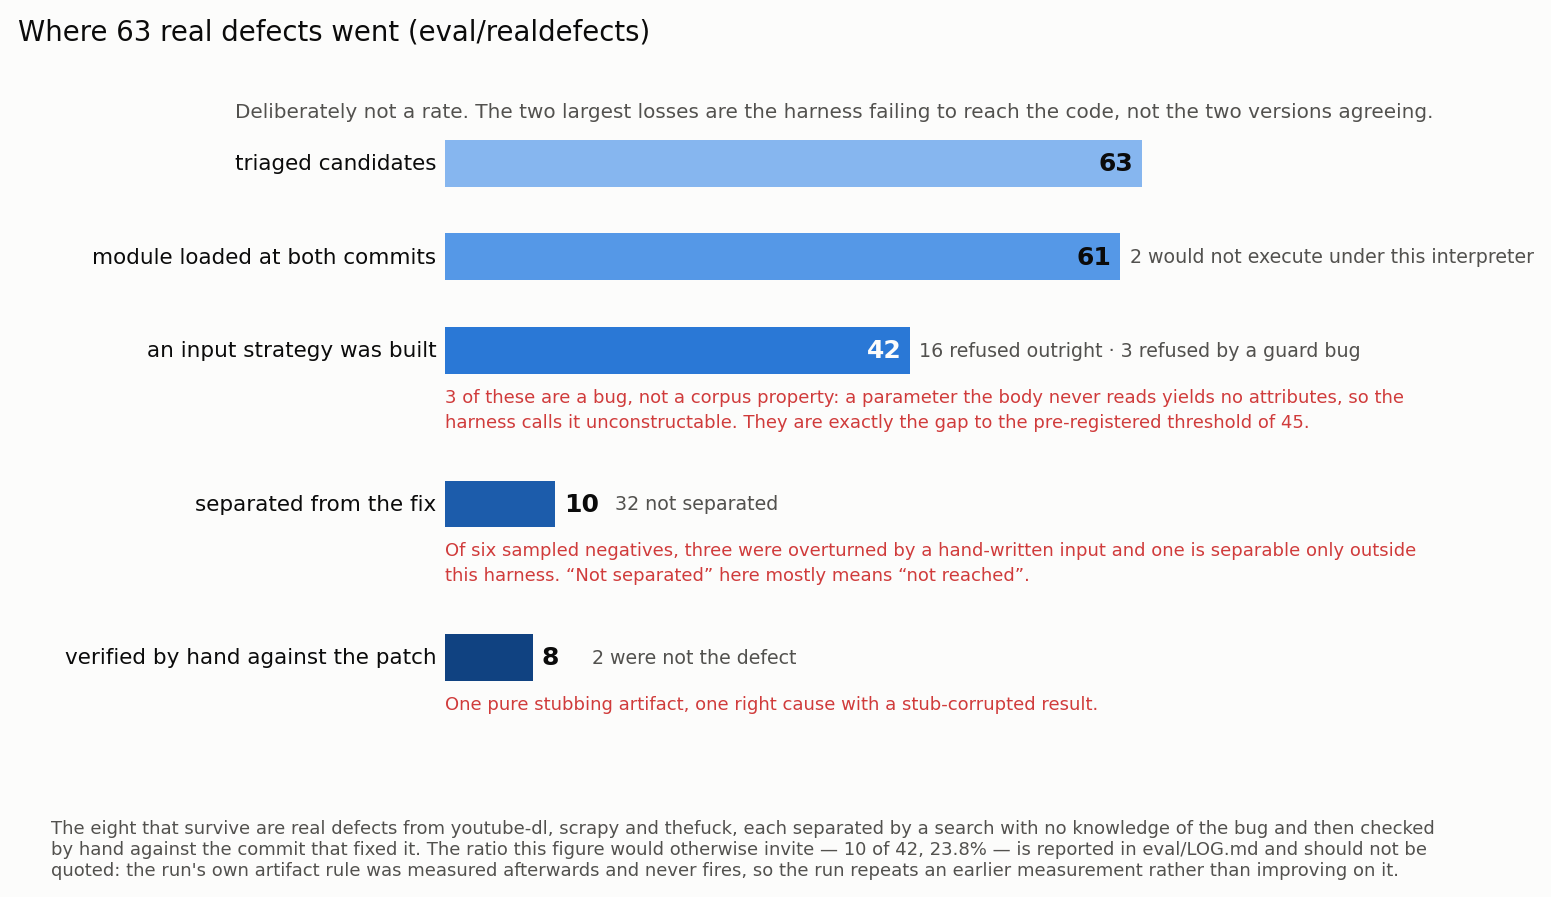
\includegraphics[width=0.86\textwidth]{fig5-realdefects.png}
  \caption{Where the real defects went. The ratio this shape invites --- separations over testable --- is the one the study's own log says not to quote, because the run's artifact rule was measured afterwards and never fires. What the figure reports is the disposition of every candidate and the eight hand-verified separations.}
  \label{fig:realdefects}
\end{figure}

\paragraph{Deployment-facing metrics.} The defined surface remains empty until a named cut: misbind, silent-fail, bleed and time-to-stage for identity; refutation, discord, miss-observed, replay-divergence and escape-replay rates for scrutiny and standing --- each with its selection biases stated beside it. A deployment still owes the two empirical studies the theorems cannot supply: coupling of its defect models to its generators' real faults, and the escape corpus's coverage of what its finders actually find.

\section{Related work}
\label{sec:related}

\paragraph{Foundations.} This stack completes Clark and Wilson's integrity model~\cite{clarkwilson} for non-replayable workers: the identity layer is their enforcement rules, the scrutiny layer their integrity verification procedure together with its certification record, and the standing layer their certification-maintenance discipline. Fail-safe defaults are Saltzer and Schroeder's~\cite{saltzer}; complete mediation, tamper-evidence and verifiability are Anderson's reference-monitor triad~\cite{anderson}, which \Cref{sec:composed,sec:method} instantiate for work products rather than for processes.

\paragraph{Scrutiny.} Measuring a suite by seeded defects is mutation analysis~\cite{demillo,jiaharman}, whose relation to real faults is the empirical question our third study attacks and does not settle~\cite{just}; industrial-scale experience is Beller et al.~\cite{beller}. Randomised checkers with declared error mass are property testing~\cite{ggr} and Freivalds' probabilistic verifiers~\cite{freivalds}; proof-carrying code~\cite{necula} is the power-one corner of the same axis. Concordance across samples is the zero-entropy gate of which semantic entropy is the graded statistic~\cite{kuhn,farquhar}; the limits of independent versions are Knight and Leveson's~\cite{knightleveson}. Self-consistency admission~\cite{chen2023} treats agreement as a soft score to maximise, where concordance here is a precondition that refuses.

\paragraph{Standing.} Eliminative argumentation and the Assurance 2.0 defeater discipline~\cite{goodenough,bloomfield} are the nearest neighbours: our escapes are their defeaters, mechanised, with a kernel-refused rather than assessor-flagged successor policy. Regression-from-escapes and mined-fault mutation are the corpus practice~\cite{tufano,beller}. The standing query's shape, and the fact that deleting a revocation raises standing, is certificate revocation~\cite{rfc5280,kocher,naor}; transparency logs and tamper-evident logging supply the length witness~\cite{laurie,crosby}; flaky-test quarantine and error budgets are demotion's fail-open ancestors. Adaptive conformal inference~\cite{gibbs} is the shape a statistical calibration theorem would have, and \Cref{sec:limits} says why it does not fit an adversarially censored escape channel.

\paragraph{The validity calculus is not ours.} \Cref{thm:asym} deserves its ancestry stated rather than left for a referee to supply. A standing predicate whose negative conjuncts are retracted when their support disappears is Doyle's out-list~\cite{doyle}; that a claim's status is a fixpoint of the record rather than an authority's act is Dung's grounded semantics~\cite{dung}; and reinstating a claim by attacking its defeater --- which is precisely the channel the first version of this kernel left open --- is Pollock's undercutting defeat~\cite{pollock}. Those three formalise the calculus. What we add is its mechanisation inside an admission kernel: the defeater is a re-run of the certifying instrument rather than an assertion, and the undercut is admitted only past a demonstration on the defeated run together with an attributed decision.

\paragraph{Deltas we do claim.} Three, stated narrowly. First, carried power as a \emph{primary} that composes only by union over a shared defect model or a labelled maximum, never a product, and whose two sorts are never collapsed --- mutation-testing practice reports a rate and composes across artifacts nowhere. Second, escapes as counterfactual re-runs of the instrument the seal already trusted, which is what makes the impeachment channel add no trust assumption; revocation infrastructures accept an authority's assertion instead, and the succession ratchet then makes forgetting a filed defect a \emph{refused transition} rather than a flagged omission. Third, \Cref{thm:asym}'s mechanisation: the two directions of a standing query carry different evidential burdens, and while the calculus is Pollock's and Dung's, we know of no prior kernel in which un-revocation of a demonstrated defeater is gated on a demonstration against that defeater plus a named act. We do \emph{not} claim novelty for impeachment, for measured scrutiny, for the validity calculus, or for the access-control skeleton.

\section{Limitations, and what is not proved}
\label{sec:limits}

\paragraph{Truth.} Survival is not correctness; impeachment's absence is not soundness; nothing in any layer says an artifact is good.

\paragraph{Coupling.} Power is exact on a named $D$ and transfers to a generator's real defects only under an empirical hypothesis (B6), stated and not proved. \Cref{sec:eval}'s third study attacks it directly, and the result is that it remains open: the differential separates eight real historical defects from their fixes, which is evidence that the mechanism reaches real faults at all, but no rate survived scrutiny and the corpus is filtered to module-level functions, so nothing about a population follows.

\paragraph{Representativeness.} The escape corpus is a selected, adversarially steerable subsample of real defects. Every aggregate built on it can be steered by parties who file only true things, and silence is unreadable except through journaled audits whose reference is the corpus itself.

\paragraph{Reports.} Harness honesty, runtime hermeticity, author identity, nonce unpredictability, byte availability and operator governance are assumptions (\Cref{app:assumptions}), with the one asymmetry the design buys: lies about deterministic components are falsifiable by replay after the fact.

\paragraph{Exposure.} A generator that has memorised a public refuter can game it. The post-artifact seed and the package exclusions narrow this; pretraining exposure is outside both, and an adaptive retry after a refutation is neither forbidden nor labelled beyond the excluded categories.

\paragraph{Consumer redirection.} The guarantees stop at the kernels' queries. A deployment whose promotion predicates read the identity store has identity guarantees only. The reference server routes promotion through \Cref{eq:pred}, with unsealable lines labelled and their reason stated; consumers outside the repository remain an obligation. That server's admission and calibration state is process-lifetime only: the kernels rebuild from their journals, but the reference server persists none of them, so a restart empties the escape ledger and everything the standing layer promises about forgetting holds within one process.

\paragraph{Record completeness.} Replay proves that the events present form a history the live machine would have accepted, not which history actually ran. See the residue in \Cref{sec:composed}, and its widening in \Cref{sec:findings}.

\paragraph{Liveness.} Nothing here makes any gate reachable. Every theorem is a safety property, and a strategy that refuses everything satisfies all of them.

\paragraph{Methodology.} Per-guard deletion proves each guard individually load-bearing; it does not prove the guard \emph{set} adequate. Violations refused only by a pair of guards need registered joint cuts, and we know of two that were missing when we looked. Citation binding is a move-detector, not a semantic check.

\section{Conclusion}

Certifying the output of a non-replayable generator by naming its author is not available. What is available is a record that cannot lie about procedure: who ran, what the artifact survived at what measured strength, and what has been found against it since. Admissible is that record with a kernel around it, and the discipline that keeps the two from drifting apart is what found five soundness defects in the kernel's own released version --- including one that let a single party un-impeach every artifact a checker had impeached. The repair produced a theorem worth stating on its own: a standing query's two directions carry different evidential burdens, and a kernel that cannot adjudicate between conflicting reports should at least refuse to let the later one win in silence.

\paragraph{Artifact availability.} The kernels, the journal event contract, every proof cited in this paper, and the three evaluation studies with their append-only run log are in the source repository~\cite{repo}. The three kernels are pure Python with no I/O and injectable clocks and nonce sources. Counts stated in \Cref{sec:method} are derived by the repository's own collection test rather than typed, because a remembered count is exactly the claim this discipline exists to catch.

\paragraph{Use of generative tools.} Portions of the manuscript and of the exploratory theory that produced the polarity computation of \Cref{sec:findings} were drafted with the assistance of large language models, and the resulting findings were then re-derived against the unmodified kernel by adversarial review before being accepted. The author takes full responsibility for all content, including every citation and every theorem statement.

\paragraph{Acknowledgements.} The adversarial review rounds described in \Cref{sec:method} were conducted with automated reviewers under the author's direction; their confirmed findings, and the ones refuted by a skeptic, are journaled in the repository.

\appendix

\section{Assumptions}
\label{app:assumptions}

Every theorem in this paper holds relative to the assumptions below. A failure of any one places the world outside the set the theorems quantify over, and they say nothing about it.

\begin{longtable}{@{}p{0.07\textwidth}p{0.88\textwidth}@{}}
\toprule
\textbf{Id} & \textbf{Identity-layer assumption} \\
\midrule
\endfirsthead
\toprule
\textbf{Id} & \textbf{Identity-layer assumption (continued)} \\
\midrule
\endhead
A0 & The allow set of a class is finite. \\
A1 & The executed model identity is the one the inference client reported for that call. \\
A2 & A watchdog outside the worker records death while a stage is running. \\
A4 & Stages are sequential; policy and author snapshots are taken at Admit. \\
A6 & On a check stage the effective allow set excludes the item's authors. \\
A7 & Admit records the specialist as tried. \\
A9 & Death is observable to the watchdog. \\
A10 & \textbf{Execution fidelity.} The adapter that reports what ran did run it. This is the trusted boundary of the identity layer. \\
A11 & The artifact hash function is second-preimage resistant against a party who chooses the bytes. \\
A12--A13 & Context packages, receipts and steering streams are reported by the harness over the bytes the kernel hashed. \\
\bottomrule
\end{longtable}

\begin{longtable}{@{}p{0.07\textwidth}p{0.88\textwidth}@{}}
\toprule
\textbf{Id} & \textbf{Scrutiny- and standing-layer assumption} \\
\midrule
\endfirsthead
\toprule
\textbf{Id} & \textbf{Scrutiny- and standing-layer assumption (continued)} \\
\midrule
\endhead
B0 & The identity layer holds underneath, and no upper transition writes its state. \\
B1 & \textbf{Harness honesty.} A verdict, witness hash, ledger, package-category set and sampling configuration are reports from a harness that ran what it names on the bytes the kernel hashed. A forged \emph{survived} on a deterministic refuter is a replay divergence when a third party re-runs it, which is more than can be said of a forged executed-model identity. \\
B2 & \textbf{Pinned hermetic runtime.} A refuter runs under a pinned toolchain with no clock, network or environment, and a runtime-counted fuel budget rather than a wall-clock deadline, so its observable is a function of version, bytes, seed and fuel. The kernel checks this only by falsification. \\
B3 & Exhaustion, crash and death are reported as \emph{inconclusive}, never as \emph{survived}. \\
B4 & The $k$ samples of a line are $k$ draws from the bind's output distribution at the declared sampling configuration. \\
B5 & A defect-model hash names one finite set of seeded defects, each shipped with a killing witness so none is equivalent to the original. \\
B6 & \textbf{Coupling.} A kill rate on a defect model is read as power against a generator's actual defects only under the coupling hypothesis. That reading is empirical and belongs to the reader; the seal carries the model's identity so the reading can be made. \\
B7 & The hash is second-preimage resistant. A collision fails toward \emph{acceptance}, so this is an assumption rather than a fail-closed property. \\
B8 & Two witnesses agree exactly when their canonical forms are byte-equal; no canonicaliser launders a syntactic difference into agreement. \\
B9 & \textbf{Nonce.} The sample nonce is drawn after the bytes are hashed and every guard has passed, and is unpredictable to the generator at generation time. \\
B10 & A seeded refuter uses exactly the seed the kernel derives. \\
B11 & \textbf{Author identity.} Author fields are declared strings the kernel compares byte for byte; that a string names the party who wrote the artifact is assumed. \\
B12 & \textbf{Post-seal byte availability.} Filing an escape requires the sealed bytes. Their loss censors the escape stream one-sidedly: it slows revocation and can never manufacture admission. \\
B13 & \textbf{Governance visibility, not governance defeat.} Budgets, gate bits, exclusions, adjudications and resolutions are operator acts. The kernel makes each a journaled, attributed, primary-carrying event; it cannot make the operator honest. \\
B14 & \textbf{Authenticated-publication boundary.} The receipt theorem assumes one authority stack, atomic single-writer transitions, an honest signer whose key is not disclosed, and an external monotone registry that cannot be rolled back with the journal. Historical authenticity begins at a trusted first anchor. \\
\bottomrule
\end{longtable}

\section{Fault tables}
\label{app:faults}

Each fault is a forbidden step. In the scrutiny layer V1--V5 are observed and publish a close; V6--V15 are guard refusals that raise and write nothing. In the standing layer E5 publishes a close, E4, E6, E7 and E9 refuse, and E1--E3 are validity semantics read at query time, so an invalid escape simply has no effect. Every fault names the method that enforces it, and \Cref{sec:method}'s deletion proofs are indexed by those methods.

\begin{longtable}{@{}p{0.06\textwidth}p{0.89\textwidth}@{}}
\toprule
\textbf{Id} & \textbf{Forbidden step (scrutiny)} \\
\midrule
\endfirsthead
\toprule
\textbf{Id} & \textbf{Forbidden step (scrutiny, continued)} \\
\midrule
\endhead
V1 & Seal after a trial on the line returned \emph{refuted}. \\
V2 & Seal with concordance below $\theta$ on any claim. \\
V3 & Seal counting an \emph{inconclusive} trial as survival. \\
V4 & Agreement recorded for a replay that diverged; measure, bound or replay on a refused refuter. \\
V5 & Seal with floor basis below $p_{\min}$, including a claim whose declared bounded figure clears the floor while its kernel-counted figure does not. \\
V6 & Sample from a stage that is not Passed, or is bound to a different specialist than the line. \\
V7 & Sample whose generator package contained an excluded category. \\
V8 & Open after a sample stage was attempted; sample $i$ after a later sample stage was attempted; trial against an unpinned claim or refuter. \\
V9 & Trial whose seed is not the kernel's derivation. \\
V10 & Seal without $k$ samples, or with a cell lacking a surviving trial. \\
V11 & Seal using a refuter with no identical replay on this line. \\
V12 & Seal using a refuter with no power record. \\
V13 & A second write to a power key; a sample beyond $k$; a second trial in one cell; a ledger id-set or record author differing from a defect model's first record. \\
V14 & A pinned refuter authored by the generator; a defect model authored by its recording refuter's author, or whose fixed author is the generator. \\
V15 & Seal of a line whose item is not accepted; a residual claiming review with no passed check stage; any write to $\SR$ other than Seal. \\
\bottomrule
\end{longtable}

\begin{longtable}{@{}p{0.06\textwidth}p{0.89\textwidth}@{}}
\toprule
\textbf{Id} & \textbf{Forbidden step (standing)} \\
\midrule
\endfirsthead
\toprule
\textbf{Id} & \textbf{Forbidden step (standing, continued)} \\
\midrule
\endhead
E1 & Effect from an escape that is not established, or whose contest was resolved \emph{void}; a filing by a checker discredited, or refused in the scrutiny registry as of the filing's own recorded cut. \\
E2 & Effect from a tier-B escape with no accepted adjudication. \\
E3 & A second charge in one cell. \\
E4 & An install whose ledger models omit a valid, unexcluded corpus entry, reference an unmeasured model, leave a claim declaration-only against a nonempty corpus, or drop a class that owes coverage. \\
E5 & Sealing under a demoted refuter where the class declared the gate. \\
E6 & A filing whose bytes do not hash to the seal's artifact hash, whose checker is not pinned (tier A), whose seed is not the kernel's derivation, or whose recorded cut precedes the seal, exceeds the journal, or moves backwards from an earlier filing's. \\
E7 & An exclusion, adjudication or resolution without a named actor and reason; a second adjudication of one escape; a second resolution of one contest; a resolution of a run nobody contested. \\
E8 & Any write to charges, corpus, exclusions or stamps except through the named transitions. \\
E9 & Any transition or budget query for a class carrying no explicit calibration policy; the budget and gate have no defaults, and an unconfigured class must never behave as an unlimited one. \\
\bottomrule
\end{longtable}

\section{Identity-layer proofs}
\label{app:identity}

Notation: a \emph{trace} is a finite sequence of transitions from the initial state, and each step applies exactly one enabled row.

\paragraph{I1 (bind integrity).} \emph{Claim:} $\mathit{pc}=\mathrm{Passed} \Rightarrow \norm(m_{\mathrm{exec}})=\norm(m_{\mathrm{decl}})=\norm(\phi(a))$. \emph{Proof:} induction on trace length. Initially $\mathit{pc}\neq\mathrm{Passed}$. The only transition setting $\mathit{pc}=\mathrm{Passed}$ is Pass, enabled only if $m_{\mathrm{exec}}$ is set and $\norm(m_{\mathrm{exec}})=\norm(m_{\mathrm{decl}})$. Now $m_{\mathrm{decl}}$ is written only by Bind, as $\phi(a)$, and no transition overwrites it before the next Admit, which also clears $m_{\mathrm{exec}}$. Hence at Pass all three agree. Observe may set $m_{\mathrm{exec}} \neq \phi(a)$; then Pass is disabled and PassRefuse is enabled, and that path never reaches Passed. $\square$

\begin{remark}
If Bind wrote $m_{\mathrm{exec}}$ the Pass guard would be tautological. Observe is what makes I1 non-vacuous, and it is the single most important structural decision in the identity layer.
\end{remark}

\paragraph{I2 (class admission).} $\mathit{pc}\in\{\mathrm{Running},\mathrm{Passed}\} \Rightarrow a \in \pi^{*}(c)\setminus\delta(c)$. \emph{Proof:} $a$ is written only by Admit, which requires $a \in \pi^{*}\setminus\delta\setminus\mathit{tried}$; Bind, Observe and Pass do not write $a$; by A4 the snapshot is the one taken at that Admit. $\square$

\paragraph{I3 (no unbound hop).} Immediate from I1 and I2. $\square$

\paragraph{I4 (frozen class and body).} After Open, $c$ and the body are constant on that item, by inspection of the write sets; a class change is a new identifier by definition. $\square$

\paragraph{I5 (accept coverage).} Accept is the only writer of $\mathit{status}=\mathrm{accepted}$ and is enabled only while the status is open and every required stage has Passed; the status guard also makes the row one-shot. $\square$

\paragraph{I6 (dual control).} By A6 the check-stage allow set excludes the authors, and Admit requires membership in it. $\square$

\paragraph{I7 (bounded admits).} A stage enables Admit at most $|\pi^{*}(c)\setminus\delta(c)|$ times: the set is finite (A0), Admit requires an untried specialist and records it as tried, so each Admit strictly decreases the remainder. The bound is on the Admit count, not on reaching Passed. $\square$

\paragraph{I8 (store only accepted).} $S$ is written only by Accept, which sets the accepted status in the same step; no writer of the status is enabled afterwards, and Open refuses an existing identifier, so the item cannot be replaced underneath the store entry. $\square$

\paragraph{I9--I17.} I9 is that a retry preserves the class, by I4. I10--I17 pin the envelope: the item freezes an attempt counter, an unpredictable nonce and a tuple of project, memory, instruction, agent, model, context-policy, tool-authority, cache-policy and steering references at Admit; Pass requires the observed package hash, attempt and nonce, executor run, latest steering continuation and executed-model receipt all to match the current envelope, so a previous-attempt receipt cannot authorise a new attempt; and project memory promotes only through a serialised compare-and-swap performed by accepted work. Each is proved by the same writer-inspection-plus-induction pattern as I1--I8, under A10--A13.

\section{Scrutiny-layer proofs}
\label{app:scrutiny}

Writer inspection, used throughout: $\SR$ is written by Seal and nowhere else, and the direct store-write entry point raises unconditionally; a power record is written only by Measure or Bound; the refusal set is written only by the refusal helper; a line's program counter becomes Sealed only in Seal and Closed only in the close helper.

\paragraph{R1 (no admission without survival).} Induction on trace length; initially $\SR=\emptyset$. The only writer of $\SR$ is Seal, enabled only past the completeness guard, which requires $k$ samples and, for every claim, every pinned refuter and every $i<k$, a trial in that cell with verdict \emph{survived}. For the second conjunct, a refuted trial closes the line in the same step, and an inconclusive one likewise; a closed line cannot Seal and nothing reopens it. Since at most one trial exists per cell, a cell holding a surviving trial holds no other. $\square$

\paragraph{R2 (power carried, never inferred).} The seal's per-refuter power is read from the power record, and the measurement guard refuses Seal if any is absent, so every figure comes from a record. Records are written only by Measure, which computes kills as the count of killed ledger entries and carries the ledger size, or by Bound, which stores the declared parameters and computes the bound in the kernel with both parameters carried into the seal. Write-once guards refuse an existing key in either mode. A seal is a frozen record written once; a later measurement on the same key is refused and on a different key does not touch the seal. The composite is the union of killed-id sets over a shared model or a labelled maximum --- both functions of records --- and the floor basis is the minimum over the sorts present, so no declared figure clears a floor a kernel-counted figure failed. $\square$

\paragraph{R3 (separation of duty, extended).} Open pins the claim snapshot and is enabled only past a guard requiring every pinned refuter to be a registry member with an author different from the generator. Membership implies declaration strictly earlier, because the declaration position is written once and the journal is append-only, so no separate ordering clause is needed and none exists. Temporal ordering against generation is enforced by reading the identity journal up to the position the kernel itself recorded --- the public row takes no position from the caller --- and refusing if any stage event for the line's first $k$ stages precedes it. The same construction at Sample refuses a sample registered after a later sample stage was attempted, so bytes cannot be assigned to slots after seeing the batch. The defect model's author is fixed by first record; a later record with a different author is refused, as is one whose author equals the recording refuter's author, and a fixed author equal to the generator is refused at both Open and Seal against the one fixed value. Package exclusion is a guard at Sample. All these hold at the step that writes the fact, nothing rewrites it, and $\SR$ is written only past all of them. $\square$

\begin{remark}
R3 forbids the refuter being shaped by the artifact. It does not forbid the artifact being shaped by a refuter the generator already knows, and it should not be cited as a theorem about specification gaming.
\end{remark}

\paragraph{R4 (concordance is a precondition).} The agreement count is computed as the number of samples whose sorted witness triples on that claim equal the designated sample's. Seal proceeds only if every claim's ratio meets $\theta$, and otherwise closes with the discord fault, naming exactly the refuters whose own witnesses differ across samples. The sealed artifact hash is the designated sample's, and the designated sample is stage $0$, fixed before any sample exists, so no transition chooses it. $\square$

\paragraph{R5, R6 (replay).} A replay compares the reported verdict and witness to the recorded pair. On inequality the refusal helper adds the key to the refusal set and closes every open line pinning it; nothing removes from that set, and measure, bound and further replay all refuse a refused refuter, while Open refuses to pin one. On equality the replay counter increments, and Seal requires, for every pinned refuter, some trial on this line with a positive counter. $\square$

\paragraph{R7--R10, R12, R13.} R7 inherits sample identity from I1--I3 by citation, since a sample is registered only against a stage that is Passed and bound to the line's generator. R8 is the accept guard at Seal plus I5 and I8. R9 and R10 are the seed derivation: the kernel hashes the bytes at Sample and draws the nonce afterwards on the live path only, so a refused sample consumes nothing, and the trial guard requires the seed to equal the kernel's derivation over that nonce and hash --- hence no seed exists before its artifact. R12 is write-once-at-Open by inspection. R13 bounds samples by $k$, trials to one per cell, and power records to one per key. $\square$

\paragraph{R11 (non-interference).} By inspection: every reference to the identity enforcer in the scrutiny module is a read, and every assignment targets scrutiny-owned state. A test additionally snapshots the identity machine's items, store, events and policy across every scrutiny transition and asserts equality. $\square$

\section{Standing-layer proofs}
\label{app:standing}

Writer inspection: a run enters the ledger in exactly one place; establishment is set in exactly one place; the discredited set grows in one place and nothing removes from it; adjudication, resolution and the contest flag are each written in exactly one place; exclusions only grow. Validity is computed at query time and never stored.

\paragraph{C1 (established, never asserted).} Every effect --- impeachment, charges, corpus membership, demotion arithmetic --- quantifies over runs passing the validity predicate, which requires establishment. Establishment is written only on a replay whose verdict and witness equal the filed pair. Filing itself is guarded: the line must be sealed and the claim in its seal (structural preconditions, since an unknown line or claim cannot be named); the verdict must be the filing kind's; the checker must be declared, not discredited, and not refused in the scrutiny registry as of the filing's own recorded cut; the kernel hashes the filed bytes itself and refuses unless they are the sealed bytes; and for tier A the seed must equal the kernel's derivation over the seal's hash and the pinned identity, so the finder authors nothing but a nonce. A tier-B escape additionally fails validity until an adjudication, which requires tier B, establishment, a named actor, a reason, and no prior decision. Rebuild re-derives the tier from the seal, re-runs the seed, standing and audit guards at the recorded cut, and requires a divergent replay to be followed by its discredit event. $\square$

\paragraph{C2 (charge totality and unit).} The charge query iterates valid refuted runs and adds, for every refuter pinned to the escaped claim in that line's seal, the cell into a set. By R1 each such refuter holds a surviving trial on the designated sample, so the cell names a journaled wrong verdict; by set semantics a second escape on the same cell adds nothing, so witness and checker multiplicity never multiply charges. No transition writes a charge: the quantity exists only as this query. $\square$

\begin{remark}
A charge is a co-liability of every refuter pinned on the claim, not a per-refuter miss certificate. A reader who wants the latter needs a per-checker query, which the kernel does not currently expose.
\end{remark}

\paragraph{C3 (\Cref{thm:asym}).} Downward, the impeachment query is a read over the filed runs and the validity predicate; no field of a seal is assignable, since seals are frozen records, and no standing transition touches the sealed store (C7). Upward, enumerate the writers of every field the validity predicate reads. Establishment falls to no transition: nothing assigns it false. The resolution field is written in exactly one place, past a guard requiring a contested and unresolved run, a decision in $\{\mathrm{uphold},\mathrm{void}\}$, and a nonempty actor and reason. The contest flag is written in exactly one place, on a replay of that same run whose reported pair diverges from the filed pair, and only when the run had already established. The adjudication field is compared for equality with \emph{accept} and gates tier B alone, so it can never turn a valid run invalid. Hence the sole path from valid to invalid is a divergent replay of the run itself followed by a \emph{void} resolution.

The two channels that formerly lifted impeachment without either --- a discredit of the checker arising from a divergence on a \emph{different} run, and a refusal entry in the scrutiny registry from a divergent trial replay on another line --- are gone with the clause that read them, and the removal is derived rather than assumed: an unestablished run already fails the establishment conjunct, so a clause voiding unestablished runs of a discredited checker is unreachable, and a clause voiding \emph{established} ones is exactly what the transition table forbade. That the kernel cannot decide which of two conflicting reports is true is B1 and B2 restated; what it can do, and now does, is refuse to let the later report win in silence. $\square$

\paragraph{C4 (the ratchet).} The install transition is the only path that drives the scrutiny layer's policy installation from this authority, and it is enabled only past three guards: every ledger claim's defect model has a kernel-fixed id-set, always satisfiable in advance since measurement reads no policy state; that id-set contains the derived defect identifier of every corpus entry not excluded, where the corpus is the valid escapes of the class minus exclusions; and a class with a nonempty net corpus cannot vanish from the incoming policy. A declaration-only claim has no model to cover with, which is why that case is refused separately. Exclusion is itself a guarded, journaled decision requiring a named actor, a reason, and valid escapes of the class. The install event carries the coverage primaries, the per-claim model map, the predecessor diff of dropped identifiers and any dropped classes. $\square$

\begin{remark}
The successor relation quantifies over journaled installs of this authority, not over a model-to-model lineage: an unrelated new model faces the identical check. A deployment that installs a policy directly on the scrutiny layer bypasses the ratchet, which is the interposition boundary stated where the paper states consumer redirection.
\end{remark}

\paragraph{C5 (track record carried, mediation provable).} The seal transition stamps immediately after the scrutiny seal returns, emitting the stamp with the primaries for every pinned refuter and the corpus provenance split. No ratio is computed anywhere, and a zero charge count is absence of filed evidence rather than measured power. Rebuild recomputes both the records and the split and refuses a stamp that does not recompute, bounding the participation count to seals at or before this seal's position so that what the live stamp saw is what rebuild recomputes. The mediation query reads the stamp back: a line is mediated exactly when one stamp exists for it and is bound to the seal's own position. Adding a second stamp, or re-pointing one, is refused on rebuild; removing the only stamp is not detectable, since an unstamped seal is what a never-mediated line looks like, but it lowers the line to layer IR and can never raise standing. A stamp appended for the most recent unmediated seal is accepted, because nothing earlier contradicts it, while one forged for any earlier seal breaks stamp order and is refused. $\square$

\paragraph{C6 (demotion).} The demotion query compares the charge count to the class's declared budget; charges are the valid cells (C2), so the crossing tracks validity exactly and no stored flag can go stale in either direction. It falls only where \Cref{thm:asym}'s upward direction allows, on a contested run resolved \emph{void}: a checker's discredit or refusal no longer lowers the count, which is the fail-closed reading, since a suspect instrument stays charged rather than being cleared by a report about itself. Open refuses a class whose current policy pins a demoted refuter, unconditionally. Seal first refuses a line that is not open --- an earlier version emitted a close event for a line that stayed sealed --- then consults the seal-gate check, which acts only where the class declared it, and on a crossing publishes the close with its fault and the refuter's primaries before closing the line through the scrutiny layer's own operator close. No standing transition iterates lines, so there is no cascade, and existing seals are untouched. Rebuild refuses a gated close whose refuter is not demoted at that point. $\square$

\paragraph{C7 (non-interference).} By inspection, every assignment in the standing module targets standing-owned state, and its only effects on the lower machines are calls to their own guarded transitions. One qualification, which we state because a review found it and the published proof sentence had been too strong: the atomicity wrapper that restores state when a standing attempt fails \emph{after} the scrutiny seal has committed does restore the scrutiny layer's line and store entries and truncate its regenerated events. C7 therefore holds at attempt granularity rather than step granularity, which is the granularity the composition results actually need. $\square$

\bibliographystyle{plain}
\bibliography{references}

\end{document}
